
	Here is a brief summarize about the changes made to adapt the previous application to the ones needed to use datasets. In case of the Ground Station (GS) application, any change is needed. Because the interface was defined in that way. As Described previously, the GS receive through a socket the information about the quad-rotors and its segmented image. This data could be provided for whoever that adapts to this interface (Simulation as previously, dataset reader, real quad-rotor, etc...) \ref{fig:Interfaces}
	
	\begin{figure}[th]
		\centering
		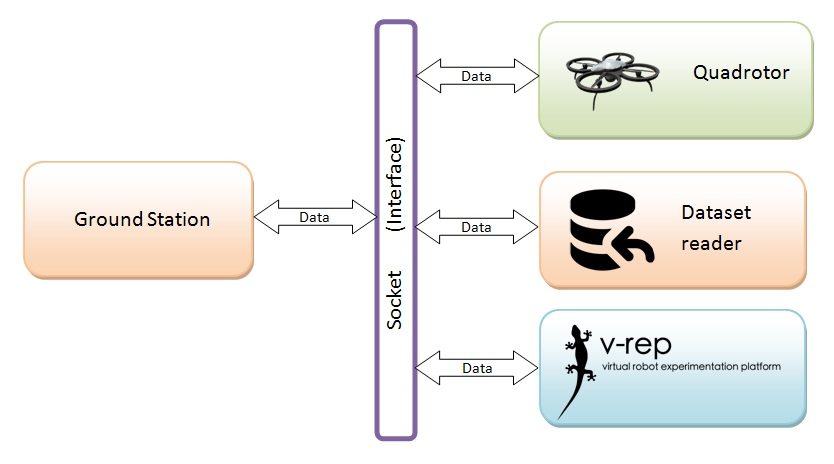
\includegraphics[width=\linewidth]{../Images/c4/Interfaces}
		\caption{Communication interface}
		\label{fig:Interfaces}
	\end{figure}

	